% IMPORTANT: add or remove (comment out) the boolean '\solutiontrue' below to
% create the solution document or the exercise document respectively.
% First we create the switch to make either the exercises or the solutions
\newif\ifsolution\solutionfalse
% To create the solution uncomment '\solutiontrue'
\solutiontrue

\documentclass[a4paper,11pt]{article}

\title{System Security,
\ifsolution Solution \else \fi
Exploits}


../author.tex

\usepackage[T1]{fontenc}
\usepackage{ae, aecompl}
\usepackage{a4wide}
\usepackage{boxedminipage}
\usepackage{graphicx}
\usepackage{subfigure}
\usepackage{enumerate}
\usepackage{url}
\usepackage{listings}
\usepackage{comment}
\usepackage{ucs}
\usepackage[utf8x]{inputenc}
\usepackage[english]{babel}

\author{Andrei Pârvu}

\ifsolution\includecomment{final}
\else\excludecomment{final}\fi

% ------------ Listings Settings
\lstset{%
  basicstyle=\small\ttfamily,
  frame=none,
  framexleftmargin=0pt,
  captionpos=b,
  showspaces=false,
  showstringspaces=false,
  showtabs=false,         
  tabsize=4,
  breaklines=true,
  breakatwhitespace=false}

% Some useful commands and environments
\newenvironment{solution}%
{\par\begin{minipage}{\linewidth}{\noindent\small\textit{Solution}\\}\begin{boxedminipage}{\linewidth}}%
{\end{boxedminipage}\end{minipage}\par\bigskip}

\begin{document}
\maketitle
\section{Metasploit: An Example Penetration Test Framework}
Given that a variety of security mechanisms that prevent memory
corruption (e.g., W$\hat{\mbox{ }}$X memory) exist, how do attacks in the
real-world work? This goal of this exercise is to give you a flavor of how
simple mistakes can be exploited using readily available tools. 

In this exercise, we will use Metasploit
(\url{http://www.metasploit.com/}) which is a penetration testing
framework that allows detection of security vulnerabilities, their
implications and the effectiveness of countermeasures. Metasploit is already
installed inside the VM, launch it using \texttt{msfconsole}.

\subsection{Pre-requisites}
Start the web-server by executing: 
\verb|su -c /usr/share/apache-tomcat-6.0.6/bin/startup.sh|
and providing the root password (\texttt{toor}).

\subsection{Goals}
The goal of the exercise is to exploit the poorly configured
web-server. More specifically, the idea is to take advantage
of the fact that the web-server can be administered using a common
username and password. In order to make the attack realistic, we
assume that we do not have access to the web-server or its configuration files
(even though they are really inside the VM).
  
Broadly, the goal of the attack will be to find this common user
name and password and then use this to obtain a shell on the target
VM. In summary, your task is to

\begin{itemize}
\item Find the port of the web server instance using a network scan tool like
nmap. The web server listens on \texttt{127.0.0.1}.\\
\textbf{DO NOT LOOK INTO THE CONFIGURATION FILES!}
\item Using metasploit:
  \begin{enumerate}
  \item Find the username and password for the web-server
    administrator
  \item Use this information to open a shell on the web-server.
  \end{enumerate}
\end{itemize}

\noindent\textbf{Notes:} You can learn how to use the metasploit framework at
\url{http://www.metasploit.com/}. Here are a few useful commands:
\begin{itemize}
\item ``search application-name'' will give you all possible exploits
  available for a given application. Try and understand which of them
  best suit your requirements. There is plenty of help out there on
  the Internet!
\item ``show options'' lists the information required for the exploit (e.g.,
  target machine, port, etc.). You might also have to change one of these
  options in case your attack overwhelms the server.

\end{itemize}

\subsection{Expected Deliverables}
A brief summary of the procedure you used to open a shell on the
server that includes the following information:
\begin{itemize}
\item What nmap commands did you use to find the port on which the
  web-server was running? How does nmap find open ports?
\ifsolution\begin{solution}
For the port discovery I used the command \texttt{nmap -sT 127.0.0.1 -p1-65000} to get
a list of open and listening ports. Nmap finds open ports by trying to establish
a TCP connection (handshake) to each of them and waiting for a response.
\end{solution}\fi
\item How did you find the username and password that the web-server
  used? What exploits did you use and how do they work?
  \ifsolution\begin{solution}
For the username and password discovery I used the $msfconsole$ with the exploit
$tomcat\_mgr\_login$. This exploit tries all combinations of users and password which
are given in a certain configuration file. After running this exploit it found the user
\texttt{syssec} and password \texttt{exercise} (as seen in Figure~\ref{fig:login}).

\end{solution}\fi

\item What did you do to open a shell? What
  exploits did you use and how do they work? What is
  the simplest defense (other than using a better username and
  password) against such an attack?
  \ifsolution\begin{solution}
For opening a shell, I used the $tomcat\_mgr\_deploy$ exploit which, given the
username and password of the tomcat server, sends a payload which allows you to
open a shell (as seen in Figure~\ref{fig:shell}).\\
The payload send by the exploit opens a connection back to the attacker's machine
which creates a meterpreter. In the meterpreter one can open a shell and have root access
to the remote machine. One way of defending against such an attack would be not to run
the Apache Tomcat server as the root user and not to give permissions to this user
to open new connections with other machines.
\end{solution}\fi
 \end{itemize}
 \textit{Remember that you have to assume that you have no access to
   the webserver!}\\
  If you want to stop the web-server when you are done with this run:\\
 \verb|su -c /usr/share/apache-tomcat-6.0.6/bin/shutdown.sh|
 

\section{Malware on Mobile Phones}
Malware on Mobile Phones and Smartphones is growing rapidly with new
possibilities offered by newer models. The goal of this exercise is to to
introduce you to some weaknesses in the Android OS that can be exploited to
breach system security. 

\begin{enumerate} [(a)]
\item Describe the major differences between malware in the mobile
  world and on user's PCs. For example, what is the aim of malware on
  the mobile phones compared to that of malware on PCs?
\ifsolution\begin{solution}
Malware on mobile phones is more focused on monetization: there is an abundance of data
and personal information to collect, which can pose a thread to its user if someone gets
access to it.\\
Malware on PCs cannot have the same effect for an ordinary user, because such personal
data isn't stored in great quantity on a PC. This type of malware focuses more on DoS
attacks or corrupting your local machine in order to be hard to use.

\end{solution}\fi

\item In the context of usage of third party applications on smart phones,
  what security mechanisms exist in the Android OS to protect against
  malicious application vendors?
\ifsolution\begin{solution}
There are several methods to protect against malicious applications \cite{MalwareDetection}:
\begin{itemize}
  \item Signature-based detection - scans the code of an application and does
  pattern matching in order to identify malicious code.
  \item Specification-based detection: employs a set of rules which are considered
  normal for an application and filters out suspicious activity
  \item Behavioural-based detection: given a database of malicious behaviour on various
  mobile platforms it tries to classify the current applications that are running on the mobile
  device.
  \item Cloud-based detection: Google automatically scans application on Google Play. Each application
  is run in an isolated environment and its behaviour is compared to known Trojans and spyware.
  Google has the possibility of uninstalling potentially dangerous applications remotely from your
  device.
\end{itemize}
\end{solution}\fi

\item What are the basic requirements for an application that wants to steal
  data? More specifically, given the list of permissions available on the
  Android OS platform, describe a pair of applications: one which is a threat
  to user privacy and another whose permissions prevent such data leakage.
\ifsolution\begin{solution}
An application which which has certain permissions such as network communication / internet
access can be dangerous as they can exploit:
\begin{enumerate}
  \item gps location: a malicious user could track your location
  \item send SMS: your phone could be used to send spam messages
  \item personal information such as address book, or, more dangerous, password or
  bank account credentials.
\end{enumerate}

Theoretically, if you don't really trust a certain application by denying it these privileges
(or at least network access) you should be safe against a basic attack.
\end{solution}\fi


\item Alice is a paranoid smart phone user and does not install applications
  that have access to her contacts and the Internet. If you were a malicious
  application developer who is interested in Alice's contacts, could you
  circumvent Alice's cautious approach? If yes, how?
\ifsolution\begin{solution}
One method to circumvent this approach is to have a malware which employs privilege
escalation techniques, mainly using root exploits. \cite{AndroidVirus}.\\
The main problem behind this type of attack is that "An application with less permissions
(a non-privileged caller) is not restricted  to access components of a more privileged application
(a privileged callee)" (the exact quote and more details can be found here \cite{PermAttack}).
\end{solution}\fi

\end{enumerate}

\begin{figure} \center
  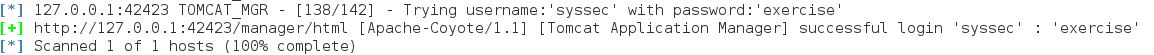
\includegraphics[width=0.9\linewidth]{login.png}
  \caption{Username and password}
  \label{fig:login}
\end{figure}
\begin{figure} \center
  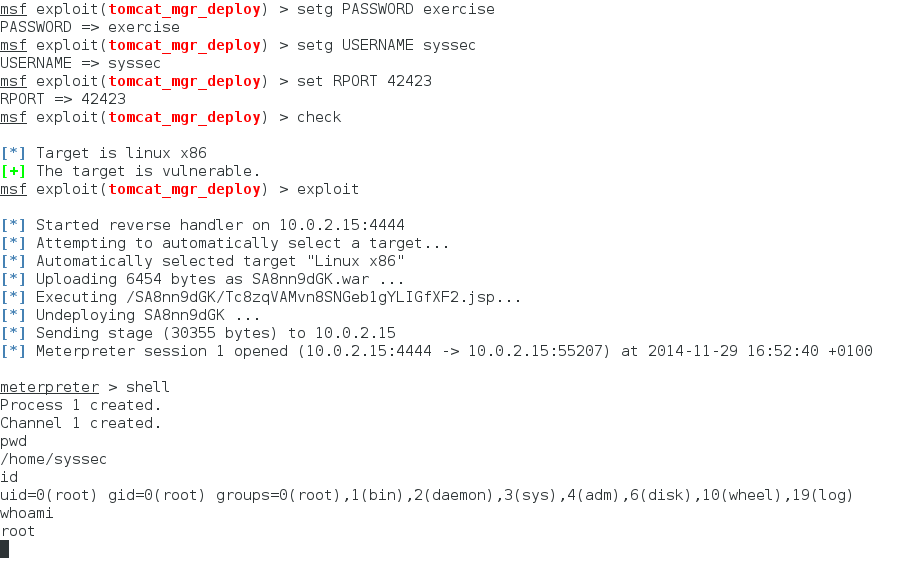
\includegraphics[width=0.8\linewidth]{shell.png}
  \caption{Shell Access}
  \label{fig:shell}
\end{figure}

\begin{thebibliography}{1}
  \bibitem{MalwareDetection} Vinit B. Mohata1, Dhananjay M. Dakhane, Ravindra L.Pardhi
    {\em Mobile Malware Detection Techniques}, 2013
  \bibitem{AndroidVirus} Rafael Fedler, Julian Schütte, Marcel Kulicke
    {\em On the Effectiveness of Malware Protection on Android}, 2013.
  \bibitem{PermAttack} Lucas Davi, Alexandra Dmitrienko, Ahmad Sadeghi, Marcel Winandy
    {\em Mobile Malware Detection Techniques}, 2013
\end{thebibliography}

\end{document}
